% !TEX root = main.tex

%%%%%%%%%%%%%%%%%%%%%%%%%%%%%%%%%%%%%%%%%%%%%%%%%%%%%%%%%%%%%%%%%%%%%%%%%%%%%%%%%%%%%%%%%%%%%%%%
\section{実験}
%%%%%%%%%%%%%%%%%%%%%%%%%%%%%%%%%%%%%%%%%%%%%%%%%%%%%%%%%%%%%%%%%%%%%%%%%%%%%%%%%%%%%%%%%%%%%%%%

\subsection{実験装置及び器具}
木製台,プローブ支持台,ガラス製水槽,平行平板電極,
静電プローブ,METRONIX MTR18-1 交流定電圧定電流電源,TEKTRONIX TBS1022
オシロスコープ,ロゴスキーコイル,抵抗$(220\si{k\Omega})$,セメント抵抗$(1\si{\Omega})$

\subsection{セットアップ}
図1のように平行平板電極を水に入れた水槽の外側に配置し,電極板に交流を印加する.
\begin{figure}[H]
    \centering
    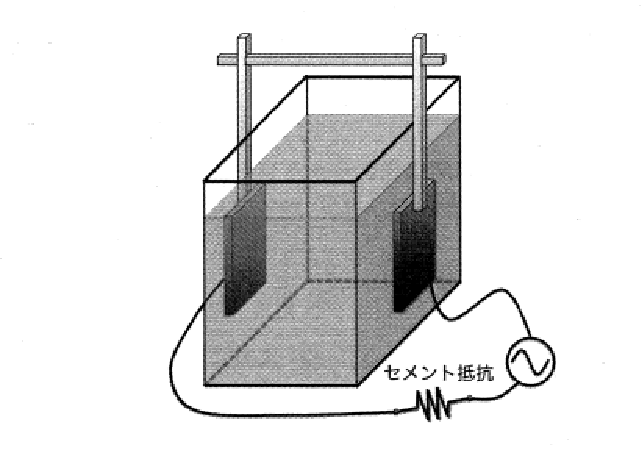
\includegraphics[scale=0.75]{figure1.pdf}
    \caption{平行平板を水槽の外に配置した場合の実験配置図}
\end{figure}

\newpage

\subsection{二本のプローブによる測定}
\begin{enumerate}
    \item 図2のように水槽に二本のプローブを差し込む.一つはプローブ支持台を用いて固定し,
    もう一つはテープで固定する.その間隔$\Delta x$は~$1\si{cm}$程度に保ち,$\Delta x$の値を測定しておく.
    \item 発振周波数は最も高い周波数$(1\si{MHz})$からスタートし,徐々に$(50\si{k}~100\si{kHz} 刻みで
    500\si{kHz}くらいまで)$周波数を下げながら実施し,それぞれの周波数における波形を記録する.
    \begin{figure}[H]
        \centering
        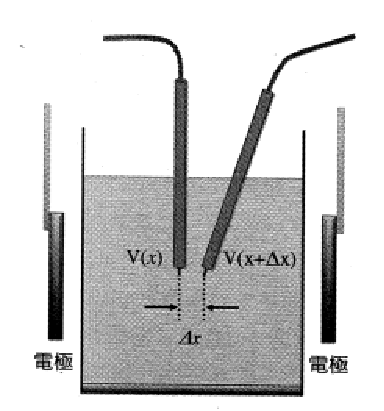
\includegraphics[scale=0.75]{figure2.pdf}
        \caption{二本プローブによる変位電流測定実験配置}
    \end{figure}
    
\end{enumerate}

\subsection{ロゴスキーコイルによる測定}
\begin{enumerate}
    \item 図3に示すように,水槽と電極板の間にロゴスキーコイルが入る程度のスペースを作り,
    そこにロゴスキーコイルを挿入する.
    \item 実験課題1と同様に発振器の周波数$\omega$を変化させながら,セメント抵抗の両端とロゴス
    キーコイルからの出力波形を記録する.
    \begin{figure}[H]
        \centering
        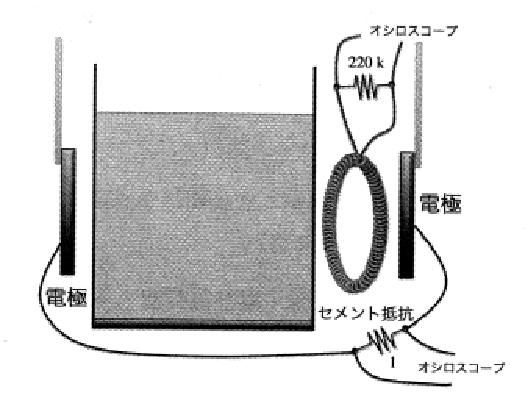
\includegraphics[scale=0.75]{figure3.pdf}
        \caption{ロゴスキーコイルによる変位電流測定実験配置}
    \end{figure}
\end{enumerate}